
% Default to the notebook output style

    


% Inherit from the specified cell style.




    
\documentclass[11pt]{article}

    
    
    \usepackage[T1]{fontenc}
    % Nicer default font (+ math font) than Computer Modern for most use cases
    \usepackage{mathpazo}

    % Basic figure setup, for now with no caption control since it's done
    % automatically by Pandoc (which extracts ![](path) syntax from Markdown).
    \usepackage{graphicx}
    % We will generate all images so they have a width \maxwidth. This means
    % that they will get their normal width if they fit onto the page, but
    % are scaled down if they would overflow the margins.
    \makeatletter
    \def\maxwidth{\ifdim\Gin@nat@width>\linewidth\linewidth
    \else\Gin@nat@width\fi}
    \makeatother
    \let\Oldincludegraphics\includegraphics
    % Set max figure width to be 80% of text width, for now hardcoded.
    \renewcommand{\includegraphics}[1]{\Oldincludegraphics[width=.8\maxwidth]{#1}}
    % Ensure that by default, figures have no caption (until we provide a
    % proper Figure object with a Caption API and a way to capture that
    % in the conversion process - todo).
    \usepackage{caption}
    \DeclareCaptionLabelFormat{nolabel}{}
    \captionsetup{labelformat=nolabel}

    \usepackage{adjustbox} % Used to constrain images to a maximum size 
    \usepackage{xcolor} % Allow colors to be defined
    \usepackage{enumerate} % Needed for markdown enumerations to work
    \usepackage{geometry} % Used to adjust the document margins
    \usepackage{amsmath} % Equations
    \usepackage{amssymb} % Equations
    \usepackage{textcomp} % defines textquotesingle
    % Hack from http://tex.stackexchange.com/a/47451/13684:
    \AtBeginDocument{%
        \def\PYZsq{\textquotesingle}% Upright quotes in Pygmentized code
    }
    \usepackage{upquote} % Upright quotes for verbatim code
    \usepackage{eurosym} % defines \euro
    \usepackage[mathletters]{ucs} % Extended unicode (utf-8) support
    \usepackage[utf8x]{inputenc} % Allow utf-8 characters in the tex document
    \usepackage{fancyvrb} % verbatim replacement that allows latex
    \usepackage{grffile} % extends the file name processing of package graphics 
                         % to support a larger range 
    % The hyperref package gives us a pdf with properly built
    % internal navigation ('pdf bookmarks' for the table of contents,
    % internal cross-reference links, web links for URLs, etc.)
    \usepackage{hyperref}
    \usepackage{longtable} % longtable support required by pandoc >1.10
    \usepackage{booktabs}  % table support for pandoc > 1.12.2
    \usepackage[inline]{enumitem} % IRkernel/repr support (it uses the enumerate* environment)
    \usepackage[normalem]{ulem} % ulem is needed to support strikethroughs (\sout)
                                % normalem makes italics be italics, not underlines
    

    
    
    % Colors for the hyperref package
    \definecolor{urlcolor}{rgb}{0,.145,.698}
    \definecolor{linkcolor}{rgb}{.71,0.21,0.01}
    \definecolor{citecolor}{rgb}{.12,.54,.11}

    % ANSI colors
    \definecolor{ansi-black}{HTML}{3E424D}
    \definecolor{ansi-black-intense}{HTML}{282C36}
    \definecolor{ansi-red}{HTML}{E75C58}
    \definecolor{ansi-red-intense}{HTML}{B22B31}
    \definecolor{ansi-green}{HTML}{00A250}
    \definecolor{ansi-green-intense}{HTML}{007427}
    \definecolor{ansi-yellow}{HTML}{DDB62B}
    \definecolor{ansi-yellow-intense}{HTML}{B27D12}
    \definecolor{ansi-blue}{HTML}{208FFB}
    \definecolor{ansi-blue-intense}{HTML}{0065CA}
    \definecolor{ansi-magenta}{HTML}{D160C4}
    \definecolor{ansi-magenta-intense}{HTML}{A03196}
    \definecolor{ansi-cyan}{HTML}{60C6C8}
    \definecolor{ansi-cyan-intense}{HTML}{258F8F}
    \definecolor{ansi-white}{HTML}{C5C1B4}
    \definecolor{ansi-white-intense}{HTML}{A1A6B2}

    % commands and environments needed by pandoc snippets
    % extracted from the output of `pandoc -s`
    \providecommand{\tightlist}{%
      \setlength{\itemsep}{0pt}\setlength{\parskip}{0pt}}
    \DefineVerbatimEnvironment{Highlighting}{Verbatim}{commandchars=\\\{\}}
    % Add ',fontsize=\small' for more characters per line
    \newenvironment{Shaded}{}{}
    \newcommand{\KeywordTok}[1]{\textcolor[rgb]{0.00,0.44,0.13}{\textbf{{#1}}}}
    \newcommand{\DataTypeTok}[1]{\textcolor[rgb]{0.56,0.13,0.00}{{#1}}}
    \newcommand{\DecValTok}[1]{\textcolor[rgb]{0.25,0.63,0.44}{{#1}}}
    \newcommand{\BaseNTok}[1]{\textcolor[rgb]{0.25,0.63,0.44}{{#1}}}
    \newcommand{\FloatTok}[1]{\textcolor[rgb]{0.25,0.63,0.44}{{#1}}}
    \newcommand{\CharTok}[1]{\textcolor[rgb]{0.25,0.44,0.63}{{#1}}}
    \newcommand{\StringTok}[1]{\textcolor[rgb]{0.25,0.44,0.63}{{#1}}}
    \newcommand{\CommentTok}[1]{\textcolor[rgb]{0.38,0.63,0.69}{\textit{{#1}}}}
    \newcommand{\OtherTok}[1]{\textcolor[rgb]{0.00,0.44,0.13}{{#1}}}
    \newcommand{\AlertTok}[1]{\textcolor[rgb]{1.00,0.00,0.00}{\textbf{{#1}}}}
    \newcommand{\FunctionTok}[1]{\textcolor[rgb]{0.02,0.16,0.49}{{#1}}}
    \newcommand{\RegionMarkerTok}[1]{{#1}}
    \newcommand{\ErrorTok}[1]{\textcolor[rgb]{1.00,0.00,0.00}{\textbf{{#1}}}}
    \newcommand{\NormalTok}[1]{{#1}}
    
    % Additional commands for more recent versions of Pandoc
    \newcommand{\ConstantTok}[1]{\textcolor[rgb]{0.53,0.00,0.00}{{#1}}}
    \newcommand{\SpecialCharTok}[1]{\textcolor[rgb]{0.25,0.44,0.63}{{#1}}}
    \newcommand{\VerbatimStringTok}[1]{\textcolor[rgb]{0.25,0.44,0.63}{{#1}}}
    \newcommand{\SpecialStringTok}[1]{\textcolor[rgb]{0.73,0.40,0.53}{{#1}}}
    \newcommand{\ImportTok}[1]{{#1}}
    \newcommand{\DocumentationTok}[1]{\textcolor[rgb]{0.73,0.13,0.13}{\textit{{#1}}}}
    \newcommand{\AnnotationTok}[1]{\textcolor[rgb]{0.38,0.63,0.69}{\textbf{\textit{{#1}}}}}
    \newcommand{\CommentVarTok}[1]{\textcolor[rgb]{0.38,0.63,0.69}{\textbf{\textit{{#1}}}}}
    \newcommand{\VariableTok}[1]{\textcolor[rgb]{0.10,0.09,0.49}{{#1}}}
    \newcommand{\ControlFlowTok}[1]{\textcolor[rgb]{0.00,0.44,0.13}{\textbf{{#1}}}}
    \newcommand{\OperatorTok}[1]{\textcolor[rgb]{0.40,0.40,0.40}{{#1}}}
    \newcommand{\BuiltInTok}[1]{{#1}}
    \newcommand{\ExtensionTok}[1]{{#1}}
    \newcommand{\PreprocessorTok}[1]{\textcolor[rgb]{0.74,0.48,0.00}{{#1}}}
    \newcommand{\AttributeTok}[1]{\textcolor[rgb]{0.49,0.56,0.16}{{#1}}}
    \newcommand{\InformationTok}[1]{\textcolor[rgb]{0.38,0.63,0.69}{\textbf{\textit{{#1}}}}}
    \newcommand{\WarningTok}[1]{\textcolor[rgb]{0.38,0.63,0.69}{\textbf{\textit{{#1}}}}}
    
    
    % Define a nice break command that doesn't care if a line doesn't already
    % exist.
    \def\br{\hspace*{\fill} \\* }
    % Math Jax compatability definitions
    \def\gt{>}
    \def\lt{<}
    % Document parameters
    \title{1. ?? ???? ???? ???}
    
    
    

    % Pygments definitions
    
\makeatletter
\def\PY@reset{\let\PY@it=\relax \let\PY@bf=\relax%
    \let\PY@ul=\relax \let\PY@tc=\relax%
    \let\PY@bc=\relax \let\PY@ff=\relax}
\def\PY@tok#1{\csname PY@tok@#1\endcsname}
\def\PY@toks#1+{\ifx\relax#1\empty\else%
    \PY@tok{#1}\expandafter\PY@toks\fi}
\def\PY@do#1{\PY@bc{\PY@tc{\PY@ul{%
    \PY@it{\PY@bf{\PY@ff{#1}}}}}}}
\def\PY#1#2{\PY@reset\PY@toks#1+\relax+\PY@do{#2}}

\expandafter\def\csname PY@tok@w\endcsname{\def\PY@tc##1{\textcolor[rgb]{0.73,0.73,0.73}{##1}}}
\expandafter\def\csname PY@tok@c\endcsname{\let\PY@it=\textit\def\PY@tc##1{\textcolor[rgb]{0.25,0.50,0.50}{##1}}}
\expandafter\def\csname PY@tok@cp\endcsname{\def\PY@tc##1{\textcolor[rgb]{0.74,0.48,0.00}{##1}}}
\expandafter\def\csname PY@tok@k\endcsname{\let\PY@bf=\textbf\def\PY@tc##1{\textcolor[rgb]{0.00,0.50,0.00}{##1}}}
\expandafter\def\csname PY@tok@kp\endcsname{\def\PY@tc##1{\textcolor[rgb]{0.00,0.50,0.00}{##1}}}
\expandafter\def\csname PY@tok@kt\endcsname{\def\PY@tc##1{\textcolor[rgb]{0.69,0.00,0.25}{##1}}}
\expandafter\def\csname PY@tok@o\endcsname{\def\PY@tc##1{\textcolor[rgb]{0.40,0.40,0.40}{##1}}}
\expandafter\def\csname PY@tok@ow\endcsname{\let\PY@bf=\textbf\def\PY@tc##1{\textcolor[rgb]{0.67,0.13,1.00}{##1}}}
\expandafter\def\csname PY@tok@nb\endcsname{\def\PY@tc##1{\textcolor[rgb]{0.00,0.50,0.00}{##1}}}
\expandafter\def\csname PY@tok@nf\endcsname{\def\PY@tc##1{\textcolor[rgb]{0.00,0.00,1.00}{##1}}}
\expandafter\def\csname PY@tok@nc\endcsname{\let\PY@bf=\textbf\def\PY@tc##1{\textcolor[rgb]{0.00,0.00,1.00}{##1}}}
\expandafter\def\csname PY@tok@nn\endcsname{\let\PY@bf=\textbf\def\PY@tc##1{\textcolor[rgb]{0.00,0.00,1.00}{##1}}}
\expandafter\def\csname PY@tok@ne\endcsname{\let\PY@bf=\textbf\def\PY@tc##1{\textcolor[rgb]{0.82,0.25,0.23}{##1}}}
\expandafter\def\csname PY@tok@nv\endcsname{\def\PY@tc##1{\textcolor[rgb]{0.10,0.09,0.49}{##1}}}
\expandafter\def\csname PY@tok@no\endcsname{\def\PY@tc##1{\textcolor[rgb]{0.53,0.00,0.00}{##1}}}
\expandafter\def\csname PY@tok@nl\endcsname{\def\PY@tc##1{\textcolor[rgb]{0.63,0.63,0.00}{##1}}}
\expandafter\def\csname PY@tok@ni\endcsname{\let\PY@bf=\textbf\def\PY@tc##1{\textcolor[rgb]{0.60,0.60,0.60}{##1}}}
\expandafter\def\csname PY@tok@na\endcsname{\def\PY@tc##1{\textcolor[rgb]{0.49,0.56,0.16}{##1}}}
\expandafter\def\csname PY@tok@nt\endcsname{\let\PY@bf=\textbf\def\PY@tc##1{\textcolor[rgb]{0.00,0.50,0.00}{##1}}}
\expandafter\def\csname PY@tok@nd\endcsname{\def\PY@tc##1{\textcolor[rgb]{0.67,0.13,1.00}{##1}}}
\expandafter\def\csname PY@tok@s\endcsname{\def\PY@tc##1{\textcolor[rgb]{0.73,0.13,0.13}{##1}}}
\expandafter\def\csname PY@tok@sd\endcsname{\let\PY@it=\textit\def\PY@tc##1{\textcolor[rgb]{0.73,0.13,0.13}{##1}}}
\expandafter\def\csname PY@tok@si\endcsname{\let\PY@bf=\textbf\def\PY@tc##1{\textcolor[rgb]{0.73,0.40,0.53}{##1}}}
\expandafter\def\csname PY@tok@se\endcsname{\let\PY@bf=\textbf\def\PY@tc##1{\textcolor[rgb]{0.73,0.40,0.13}{##1}}}
\expandafter\def\csname PY@tok@sr\endcsname{\def\PY@tc##1{\textcolor[rgb]{0.73,0.40,0.53}{##1}}}
\expandafter\def\csname PY@tok@ss\endcsname{\def\PY@tc##1{\textcolor[rgb]{0.10,0.09,0.49}{##1}}}
\expandafter\def\csname PY@tok@sx\endcsname{\def\PY@tc##1{\textcolor[rgb]{0.00,0.50,0.00}{##1}}}
\expandafter\def\csname PY@tok@m\endcsname{\def\PY@tc##1{\textcolor[rgb]{0.40,0.40,0.40}{##1}}}
\expandafter\def\csname PY@tok@gh\endcsname{\let\PY@bf=\textbf\def\PY@tc##1{\textcolor[rgb]{0.00,0.00,0.50}{##1}}}
\expandafter\def\csname PY@tok@gu\endcsname{\let\PY@bf=\textbf\def\PY@tc##1{\textcolor[rgb]{0.50,0.00,0.50}{##1}}}
\expandafter\def\csname PY@tok@gd\endcsname{\def\PY@tc##1{\textcolor[rgb]{0.63,0.00,0.00}{##1}}}
\expandafter\def\csname PY@tok@gi\endcsname{\def\PY@tc##1{\textcolor[rgb]{0.00,0.63,0.00}{##1}}}
\expandafter\def\csname PY@tok@gr\endcsname{\def\PY@tc##1{\textcolor[rgb]{1.00,0.00,0.00}{##1}}}
\expandafter\def\csname PY@tok@ge\endcsname{\let\PY@it=\textit}
\expandafter\def\csname PY@tok@gs\endcsname{\let\PY@bf=\textbf}
\expandafter\def\csname PY@tok@gp\endcsname{\let\PY@bf=\textbf\def\PY@tc##1{\textcolor[rgb]{0.00,0.00,0.50}{##1}}}
\expandafter\def\csname PY@tok@go\endcsname{\def\PY@tc##1{\textcolor[rgb]{0.53,0.53,0.53}{##1}}}
\expandafter\def\csname PY@tok@gt\endcsname{\def\PY@tc##1{\textcolor[rgb]{0.00,0.27,0.87}{##1}}}
\expandafter\def\csname PY@tok@err\endcsname{\def\PY@bc##1{\setlength{\fboxsep}{0pt}\fcolorbox[rgb]{1.00,0.00,0.00}{1,1,1}{\strut ##1}}}
\expandafter\def\csname PY@tok@kc\endcsname{\let\PY@bf=\textbf\def\PY@tc##1{\textcolor[rgb]{0.00,0.50,0.00}{##1}}}
\expandafter\def\csname PY@tok@kd\endcsname{\let\PY@bf=\textbf\def\PY@tc##1{\textcolor[rgb]{0.00,0.50,0.00}{##1}}}
\expandafter\def\csname PY@tok@kn\endcsname{\let\PY@bf=\textbf\def\PY@tc##1{\textcolor[rgb]{0.00,0.50,0.00}{##1}}}
\expandafter\def\csname PY@tok@kr\endcsname{\let\PY@bf=\textbf\def\PY@tc##1{\textcolor[rgb]{0.00,0.50,0.00}{##1}}}
\expandafter\def\csname PY@tok@bp\endcsname{\def\PY@tc##1{\textcolor[rgb]{0.00,0.50,0.00}{##1}}}
\expandafter\def\csname PY@tok@fm\endcsname{\def\PY@tc##1{\textcolor[rgb]{0.00,0.00,1.00}{##1}}}
\expandafter\def\csname PY@tok@vc\endcsname{\def\PY@tc##1{\textcolor[rgb]{0.10,0.09,0.49}{##1}}}
\expandafter\def\csname PY@tok@vg\endcsname{\def\PY@tc##1{\textcolor[rgb]{0.10,0.09,0.49}{##1}}}
\expandafter\def\csname PY@tok@vi\endcsname{\def\PY@tc##1{\textcolor[rgb]{0.10,0.09,0.49}{##1}}}
\expandafter\def\csname PY@tok@vm\endcsname{\def\PY@tc##1{\textcolor[rgb]{0.10,0.09,0.49}{##1}}}
\expandafter\def\csname PY@tok@sa\endcsname{\def\PY@tc##1{\textcolor[rgb]{0.73,0.13,0.13}{##1}}}
\expandafter\def\csname PY@tok@sb\endcsname{\def\PY@tc##1{\textcolor[rgb]{0.73,0.13,0.13}{##1}}}
\expandafter\def\csname PY@tok@sc\endcsname{\def\PY@tc##1{\textcolor[rgb]{0.73,0.13,0.13}{##1}}}
\expandafter\def\csname PY@tok@dl\endcsname{\def\PY@tc##1{\textcolor[rgb]{0.73,0.13,0.13}{##1}}}
\expandafter\def\csname PY@tok@s2\endcsname{\def\PY@tc##1{\textcolor[rgb]{0.73,0.13,0.13}{##1}}}
\expandafter\def\csname PY@tok@sh\endcsname{\def\PY@tc##1{\textcolor[rgb]{0.73,0.13,0.13}{##1}}}
\expandafter\def\csname PY@tok@s1\endcsname{\def\PY@tc##1{\textcolor[rgb]{0.73,0.13,0.13}{##1}}}
\expandafter\def\csname PY@tok@mb\endcsname{\def\PY@tc##1{\textcolor[rgb]{0.40,0.40,0.40}{##1}}}
\expandafter\def\csname PY@tok@mf\endcsname{\def\PY@tc##1{\textcolor[rgb]{0.40,0.40,0.40}{##1}}}
\expandafter\def\csname PY@tok@mh\endcsname{\def\PY@tc##1{\textcolor[rgb]{0.40,0.40,0.40}{##1}}}
\expandafter\def\csname PY@tok@mi\endcsname{\def\PY@tc##1{\textcolor[rgb]{0.40,0.40,0.40}{##1}}}
\expandafter\def\csname PY@tok@il\endcsname{\def\PY@tc##1{\textcolor[rgb]{0.40,0.40,0.40}{##1}}}
\expandafter\def\csname PY@tok@mo\endcsname{\def\PY@tc##1{\textcolor[rgb]{0.40,0.40,0.40}{##1}}}
\expandafter\def\csname PY@tok@ch\endcsname{\let\PY@it=\textit\def\PY@tc##1{\textcolor[rgb]{0.25,0.50,0.50}{##1}}}
\expandafter\def\csname PY@tok@cm\endcsname{\let\PY@it=\textit\def\PY@tc##1{\textcolor[rgb]{0.25,0.50,0.50}{##1}}}
\expandafter\def\csname PY@tok@cpf\endcsname{\let\PY@it=\textit\def\PY@tc##1{\textcolor[rgb]{0.25,0.50,0.50}{##1}}}
\expandafter\def\csname PY@tok@c1\endcsname{\let\PY@it=\textit\def\PY@tc##1{\textcolor[rgb]{0.25,0.50,0.50}{##1}}}
\expandafter\def\csname PY@tok@cs\endcsname{\let\PY@it=\textit\def\PY@tc##1{\textcolor[rgb]{0.25,0.50,0.50}{##1}}}

\def\PYZbs{\char`\\}
\def\PYZus{\char`\_}
\def\PYZob{\char`\{}
\def\PYZcb{\char`\}}
\def\PYZca{\char`\^}
\def\PYZam{\char`\&}
\def\PYZlt{\char`\<}
\def\PYZgt{\char`\>}
\def\PYZsh{\char`\#}
\def\PYZpc{\char`\%}
\def\PYZdl{\char`\$}
\def\PYZhy{\char`\-}
\def\PYZsq{\char`\'}
\def\PYZdq{\char`\"}
\def\PYZti{\char`\~}
% for compatibility with earlier versions
\def\PYZat{@}
\def\PYZlb{[}
\def\PYZrb{]}
\makeatother


    % Exact colors from NB
    \definecolor{incolor}{rgb}{0.0, 0.0, 0.5}
    \definecolor{outcolor}{rgb}{0.545, 0.0, 0.0}



    
    % Prevent overflowing lines due to hard-to-break entities
    \sloppy 
    % Setup hyperref package
    \hypersetup{
      breaklinks=true,  % so long urls are correctly broken across lines
      colorlinks=true,
      urlcolor=urlcolor,
      linkcolor=linkcolor,
      citecolor=citecolor,
      }
    % Slightly bigger margins than the latex defaults
    
    \geometry{verbose,tmargin=1in,bmargin=1in,lmargin=1in,rmargin=1in}
    
    

    \begin{document}
    
    
    \maketitle
    
    

    
    \hypertarget{uxc5b4uxb5a4-uxace0uxac1duxb4e4uxc774-uxb5a0uxb098uxac00uxace0-uxc788uxb294uxac00}{%
\section{어떤 고객들이 떠나가고
있는가?}\label{uxc5b4uxb5a4-uxace0uxac1duxb4e4uxc774-uxb5a0uxb098uxac00uxace0-uxc788uxb294uxac00}}

\hypertarget{uxac8cuxc784-uxac1cuxbc1c-uxd68cuxc0ac-auxae30uxc5c5uxc758-uxc720uxc800uxc218uxac00-uxc904uxace0-uxc788uxc74c.-94185uxba85uxc5d0uxc11c-76175uxba85uxc73cuxb85c-uxac10uxc18cuxd568}{%
\paragraph{게임 개발 회사 A기업의 유저수가 줄고 있음. 94,185명에서
76,175명으로
감소함}\label{uxac8cuxc784-uxac1cuxbc1c-uxd68cuxc0ac-auxae30uxc5c5uxc758-uxc720uxc800uxc218uxac00-uxc904uxace0-uxc788uxc74c.-94185uxba85uxc5d0uxc11c-76175uxba85uxc73cuxb85c-uxac10uxc18cuxd568}}

\begin{itemize}
\tightlist
\item
  광고: 지난 달과 비교했을 때 광고 집행은 변함이 없음
\item
  기획: 매주, 매월 시행하고 있는 게임 속 이벤트 역시 변함이 없음
  \#\#\#\# 이유가 무엇일까? 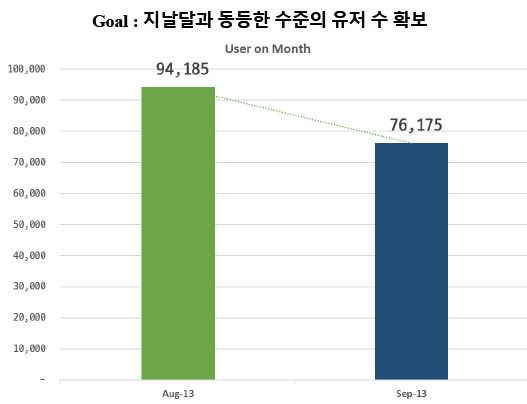
\includegraphics{1-1.jpg} \#\#\#\# 유력가설:
  성별 혹은 연령 등 특정 유저 층에서 탈퇴한 유저가 많다. \#\#\#\#
  해결책: 성별 연령별로 유저 변화수를 살펴보자.
\end{itemize}

    \hypertarget{loading-data}{%
\subsection{1. Loading data}\label{loading-data}}

    \hypertarget{uxd544uxc694uxd55c-uxb77cuxc774uxbe0cuxb7ecuxb9acuxb4e4uxc744-uxd638uxcd9c}{%
\paragraph{1) 필요한 라이브러리들을
호출}\label{uxd544uxc694uxd55c-uxb77cuxc774uxbe0cuxb7ecuxb9acuxb4e4uxc744-uxd638uxcd9c}}

    \begin{Verbatim}[commandchars=\\\{\}]
{\color{incolor}In [{\color{incolor}1}]:} \PY{c+c1}{\PYZsh{}데이터 분석에 필요한 패키지들을 파이썬으로 호출}
        \PY{k+kn}{import} \PY{n+nn}{pandas} \PY{k}{as} \PY{n+nn}{pd}
        \PY{k+kn}{import} \PY{n+nn}{os}
        \PY{k+kn}{import} \PY{n+nn}{numpy} \PY{k}{as} \PY{n+nn}{np}
        \PY{k+kn}{import} \PY{n+nn}{matplotlib}\PY{n+nn}{.}\PY{n+nn}{pyplot} \PY{k}{as} \PY{n+nn}{plt}
        \PY{o}{\PYZpc{}}\PY{k}{matplotlib} inline
        \PY{k+kn}{import} \PY{n+nn}{seaborn} \PY{k}{as} \PY{n+nn}{sns}
\end{Verbatim}


    \hypertarget{uxac01-uxbcc0uxc218uxbcc4uxb85c-uxb370uxc774uxd130-uxd560uxb2f9}{%
\paragraph{2) 각 변수별로 데이터
할당}\label{uxac01-uxbcc0uxc218uxbcc4uxb85c-uxb370uxc774uxd130-uxd560uxb2f9}}

    \begin{Verbatim}[commandchars=\\\{\}]
{\color{incolor}In [{\color{incolor}4}]:} \PY{n}{dau} \PY{o}{=} \PY{n}{pd}\PY{o}{.}\PY{n}{read\PYZus{}csv}\PY{p}{(}\PY{l+s+s2}{\PYZdq{}}\PY{l+s+s2}{dau.csv}\PY{l+s+s2}{\PYZdq{}}\PY{p}{,} \PY{n}{sep}\PY{o}{=}\PY{l+s+s2}{\PYZdq{}}\PY{l+s+s2}{,}\PY{l+s+s2}{\PYZdq{}}\PY{p}{)}
        \PY{n}{user} \PY{o}{=} \PY{n}{pd}\PY{o}{.}\PY{n}{read\PYZus{}csv}\PY{p}{(}\PY{l+s+s2}{\PYZdq{}}\PY{l+s+s2}{user\PYZus{}info.csv}\PY{l+s+s2}{\PYZdq{}}\PY{p}{,} \PY{n}{sep}\PY{o}{=}\PY{l+s+s2}{\PYZdq{}}\PY{l+s+s2}{,}\PY{l+s+s2}{\PYZdq{}}\PY{p}{)}
\end{Verbatim}


    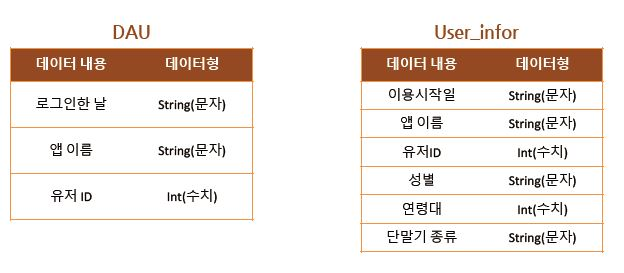
\includegraphics{1-2.jpg}

    \hypertarget{uxd638uxcd9cuxb41c-uxb370uxc774uxd130-uxc815uxbcf4-uxd655uxc778}{%
\paragraph{3) 호출된 데이터 정보
확인}\label{uxd638uxcd9cuxb41c-uxb370uxc774uxd130-uxc815uxbcf4-uxd655uxc778}}

    \begin{Verbatim}[commandchars=\\\{\}]
{\color{incolor}In [{\color{incolor}22}]:} \PY{c+c1}{\PYZsh{} 로그인해서 활동하는 날 생기는 로그 데이터}
         \PY{n}{dau}\PY{o}{.}\PY{n}{head}\PY{p}{(}\PY{p}{)}
\end{Verbatim}


\begin{Verbatim}[commandchars=\\\{\}]
{\color{outcolor}Out[{\color{outcolor}22}]:}      log\_date app\_name  user\_id
         0  2017-08-01  game-01    33754
         1  2017-08-01  game-01    28598
         2  2017-08-01  game-01    30306
         3  2017-08-01  game-01      117
         4  2017-08-01  game-01     6605
\end{Verbatim}
            
    \begin{Verbatim}[commandchars=\\\{\}]
{\color{incolor}In [{\color{incolor}24}]:} \PY{c+c1}{\PYZsh{} 가입한 사용자정보 데이터}
         \PY{n}{user}\PY{o}{.}\PY{n}{head}\PY{p}{(}\PY{p}{)}
\end{Verbatim}


\begin{Verbatim}[commandchars=\\\{\}]
{\color{outcolor}Out[{\color{outcolor}24}]:}   install\_date app\_name  user\_id gender  generation device\_type
         0   2017-04-15  game-01        1      M          40         iOS
         1   2017-04-15  game-01        2      M          10     Android
         2   2017-04-15  game-01        3      F          40         iOS
         3   2017-04-15  game-01        4      M          10     Android
         4   2017-04-15  game-01        5      M          40         iOS
\end{Verbatim}
            
    \hypertarget{data-cleaning}{%
\section{2. Data cleaning}\label{data-cleaning}}

    \hypertarget{uxac01-uxb370uxc774uxd130uxb4e4uxc744-uxacb0uxd569}{%
\paragraph{1) 각 데이터들을
결합}\label{uxac01-uxb370uxc774uxd130uxb4e4uxc744-uxacb0uxd569}}

    \begin{Verbatim}[commandchars=\\\{\}]
{\color{incolor}In [{\color{incolor}29}]:} \PY{c+c1}{\PYZsh{} Dau 데이터에 user 데이터를 결합하기}
         \PY{n}{DauUser} \PY{o}{=} \PY{n}{dau}\PY{o}{.}\PY{n}{merge}\PY{p}{(}\PY{n}{user}\PY{p}{,} \PY{n}{on}\PY{o}{=}\PY{p}{[}\PY{l+s+s2}{\PYZdq{}}\PY{l+s+s2}{user\PYZus{}id}\PY{l+s+s2}{\PYZdq{}}\PY{p}{,} \PY{l+s+s2}{\PYZdq{}}\PY{l+s+s2}{app\PYZus{}name}\PY{l+s+s2}{\PYZdq{}}\PY{p}{]}\PY{p}{)}
         \PY{n}{DauUser}\PY{o}{.}\PY{n}{head}\PY{p}{(}\PY{p}{)}
\end{Verbatim}


\begin{Verbatim}[commandchars=\\\{\}]
{\color{outcolor}Out[{\color{outcolor}29}]:}      log\_date app\_name  user\_id install\_date gender  generation device\_type
         0  2017-08-01  game-01    33754   2017-08-01      M          20         iOS
         1  2017-08-02  game-01    33754   2017-08-01      M          20         iOS
         2  2017-08-01  game-01    28598   2017-07-16      M          50         iOS
         3  2017-08-04  game-01    28598   2017-07-16      M          50         iOS
         4  2017-08-12  game-01    28598   2017-07-16      M          50         iOS
\end{Verbatim}
            
    \hypertarget{uxc6d4uxbcc4-uxc815uxb82cuxc744-uxc704uxd55c-uxbb38uxc790-uxcc98uxb9ac}{%
\paragraph{2)월별 정렬을 위한 문자
처리}\label{uxc6d4uxbcc4-uxc815uxb82cuxc744-uxc704uxd55c-uxbb38uxc790-uxcc98uxb9ac}}

    \begin{Verbatim}[commandchars=\\\{\}]
{\color{incolor}In [{\color{incolor}30}]:} \PY{c+c1}{\PYZsh{}일자 데이터 중 \PYZsq{}월\PYZsq{}을 떼어내 별도의 열로 저장}
         \PY{n}{DauUser}\PY{p}{[}\PY{l+s+s1}{\PYZsq{}}\PY{l+s+s1}{log\PYZus{}month}\PY{l+s+s1}{\PYZsq{}}\PY{p}{]} \PY{o}{=} \PY{n}{DauUser}\PY{p}{[}\PY{l+s+s1}{\PYZsq{}}\PY{l+s+s1}{log\PYZus{}date}\PY{l+s+s1}{\PYZsq{}}\PY{p}{]}\PY{o}{.}\PY{n}{str}\PY{p}{[}\PY{p}{:}\PY{l+m+mi}{7}\PY{p}{]}
         \PY{n}{DauUser}\PY{p}{[}\PY{p}{:}\PY{l+m+mi}{5}\PY{p}{]}
\end{Verbatim}


\begin{Verbatim}[commandchars=\\\{\}]
{\color{outcolor}Out[{\color{outcolor}30}]:}      log\_date app\_name  user\_id install\_date gender  generation device\_type  \textbackslash{}
         0  2017-08-01  game-01    33754   2017-08-01      M          20         iOS   
         1  2017-08-02  game-01    33754   2017-08-01      M          20         iOS   
         2  2017-08-01  game-01    28598   2017-07-16      M          50         iOS   
         3  2017-08-04  game-01    28598   2017-07-16      M          50         iOS   
         4  2017-08-12  game-01    28598   2017-07-16      M          50         iOS   
         
           log\_month  
         0   2017-08  
         1   2017-08  
         2   2017-08  
         3   2017-08  
         4   2017-08  
\end{Verbatim}
            
    \hypertarget{data-analysis}{%
\section{3. Data analysis}\label{data-analysis}}

    \hypertarget{uxd06cuxb85cuxc2a4-uxc9d1uxacc4uxb97c-uxc774uxc6a9uxd55c-uxbd84uxc11d}{%
\paragraph{1)크로스 집계를 이용한
분석}\label{uxd06cuxb85cuxc2a4-uxc9d1uxacc4uxb97c-uxc774uxc6a9uxd55c-uxbd84uxc11d}}

    \hypertarget{uxc131uxbcc4uxc5d0-uxb530uxb978-uxc811uxc18d-uxc77cuxc790}{%
\paragraph{성별에 따른 접속
일자}\label{uxc131uxbcc4uxc5d0-uxb530uxb978-uxc811uxc18d-uxc77cuxc790}}

    \begin{Verbatim}[commandchars=\\\{\}]
{\color{incolor}In [{\color{incolor}31}]:} \PY{n}{pd}\PY{o}{.}\PY{n}{crosstab}\PY{p}{(}\PY{n}{DauUser}\PY{p}{[}\PY{l+s+s2}{\PYZdq{}}\PY{l+s+s2}{log\PYZus{}month}\PY{l+s+s2}{\PYZdq{}}\PY{p}{]}\PY{p}{,} \PY{n}{DauUser}\PY{p}{[}\PY{l+s+s2}{\PYZdq{}}\PY{l+s+s2}{gender}\PY{l+s+s2}{\PYZdq{}}\PY{p}{]}\PY{p}{)}
\end{Verbatim}


\begin{Verbatim}[commandchars=\\\{\}]
{\color{outcolor}Out[{\color{outcolor}31}]:} gender         F      M
         log\_month              
         2017-08    47358  46849
         2017-09    38041  38150
\end{Verbatim}
            
    \hypertarget{uxc5f0uxb839uxc5d0-uxb530uxb978-uxc811uxc18duxc77cuxc790}{%
\paragraph{연령에 따른
접속일자}\label{uxc5f0uxb839uxc5d0-uxb530uxb978-uxc811uxc18duxc77cuxc790}}

    \begin{Verbatim}[commandchars=\\\{\}]
{\color{incolor}In [{\color{incolor}32}]:} \PY{n}{pd}\PY{o}{.}\PY{n}{crosstab}\PY{p}{(}\PY{n}{DauUser}\PY{p}{[}\PY{l+s+s2}{\PYZdq{}}\PY{l+s+s2}{log\PYZus{}month}\PY{l+s+s2}{\PYZdq{}}\PY{p}{]}\PY{p}{,} \PY{n}{DauUser}\PY{p}{[}\PY{l+s+s2}{\PYZdq{}}\PY{l+s+s2}{generation}\PY{l+s+s2}{\PYZdq{}}\PY{p}{]}\PY{p}{)}
\end{Verbatim}


\begin{Verbatim}[commandchars=\\\{\}]
{\color{outcolor}Out[{\color{outcolor}32}]:} generation     10     20     30    40    50
         log\_month                                  
         2017-08     18786  33682  28080  8830  4829
         2017-09     15392  27241  22229  7494  3835
\end{Verbatim}
            
    \hypertarget{uxc131uxbcc4-uxc5f0uxb839uxc5d0-uxb530uxb978-uxc811uxc18duxc77cuxc790---uxccab-uxbc88uxc9f8-uxbc29uxbc95}{%
\paragraph{성별-연령에 따른 접속일자 - 첫 번째
방법}\label{uxc131uxbcc4-uxc5f0uxb839uxc5d0-uxb530uxb978-uxc811uxc18duxc77cuxc790---uxccab-uxbc88uxc9f8-uxbc29uxbc95}}

    \begin{Verbatim}[commandchars=\\\{\}]
{\color{incolor}In [{\color{incolor}33}]:} \PY{n}{pd}\PY{o}{.}\PY{n}{crosstab}\PY{p}{(}\PY{n}{DauUser}\PY{p}{[}\PY{l+s+s2}{\PYZdq{}}\PY{l+s+s2}{log\PYZus{}month}\PY{l+s+s2}{\PYZdq{}}\PY{p}{]}\PY{p}{,} \PY{n}{columns}\PY{o}{=}\PY{p}{[}\PY{n}{DauUser}\PY{p}{[}\PY{l+s+s2}{\PYZdq{}}\PY{l+s+s2}{gender}\PY{l+s+s2}{\PYZdq{}}\PY{p}{]}\PY{p}{,} \PY{n}{DauUser}\PY{p}{[}\PY{l+s+s2}{\PYZdq{}}\PY{l+s+s2}{generation}\PY{l+s+s2}{\PYZdq{}}\PY{p}{]}\PY{p}{]}\PY{p}{)}
\end{Verbatim}


\begin{Verbatim}[commandchars=\\\{\}]
{\color{outcolor}Out[{\color{outcolor}33}]:} gender         F                               M                          
         generation    10     20     30    40    50    10     20     30    40    50
         log\_month                                                                 
         2017-08     9091  17192  14219  4599  2257  9695  16490  13861  4231  2572
         2017-09     7316  13628  11460  3856  1781  8076  13613  10769  3638  2054
\end{Verbatim}
            
    \hypertarget{uxb514uxbc14uxc774uxc2a4-uxc720uxd615uxc5d0-uxb530uxb978-uxc811uxc18duxc77cuxc790}{%
\paragraph{디바이스 유형에 따른
접속일자}\label{uxb514uxbc14uxc774uxc2a4-uxc720uxd615uxc5d0-uxb530uxb978-uxc811uxc18duxc77cuxc790}}

    \begin{Verbatim}[commandchars=\\\{\}]
{\color{incolor}In [{\color{incolor}35}]:} \PY{n}{pd}\PY{o}{.}\PY{n}{crosstab}\PY{p}{(}\PY{n}{DauUser}\PY{p}{[}\PY{l+s+s2}{\PYZdq{}}\PY{l+s+s2}{log\PYZus{}month}\PY{l+s+s2}{\PYZdq{}}\PY{p}{]}\PY{p}{,} \PY{n}{DauUser}\PY{p}{[}\PY{l+s+s2}{\PYZdq{}}\PY{l+s+s2}{device\PYZus{}type}\PY{l+s+s2}{\PYZdq{}}\PY{p}{]}\PY{p}{)}
\end{Verbatim}


\begin{Verbatim}[commandchars=\\\{\}]
{\color{outcolor}Out[{\color{outcolor}35}]:} device\_type  Android    iOS
         log\_month                  
         2017-08        46990  47217
         2017-09        29659  46532
\end{Verbatim}
            
    \hypertarget{data-visualization}{%
\section{4. Data Visualization}\label{data-visualization}}

    \hypertarget{uxb514uxbc14uxc774uxc2a4-uxc720uxd615uxbcc4-uxc811uxc18duxc77cuxc790uxc758-uxc2dcuxac01uxd654---uxb77cuxc778-uxadf8uxb798uxd504}{%
\paragraph{1) 디바이스 유형별 접속일자의 시각화 - 라인
그래프}\label{uxb514uxbc14uxc774uxc2a4-uxc720uxd615uxbcc4-uxc811uxc18duxc77cuxc790uxc758-uxc2dcuxac01uxd654---uxb77cuxc778-uxadf8uxb798uxd504}}

    \begin{Verbatim}[commandchars=\\\{\}]
{\color{incolor}In [{\color{incolor}38}]:} \PY{n}{data} \PY{o}{=} \PY{n}{pd}\PY{o}{.}\PY{n}{crosstab}\PY{p}{(}\PY{n}{DauUser}\PY{p}{[}\PY{l+s+s2}{\PYZdq{}}\PY{l+s+s2}{log\PYZus{}date}\PY{l+s+s2}{\PYZdq{}}\PY{p}{]}\PY{p}{,} \PY{n}{DauUser}\PY{p}{[}\PY{l+s+s2}{\PYZdq{}}\PY{l+s+s2}{device\PYZus{}type}\PY{l+s+s2}{\PYZdq{}}\PY{p}{]}\PY{p}{)}
\end{Verbatim}


    \begin{Verbatim}[commandchars=\\\{\}]
{\color{incolor}In [{\color{incolor}39}]:} \PY{n}{graph} \PY{o}{=} \PY{n}{pd}\PY{o}{.}\PY{n}{DataFrame}\PY{p}{(}\PY{n}{data}\PY{p}{)}
         \PY{n}{graph}\PY{o}{.}\PY{n}{plot}\PY{o}{.}\PY{n}{line}\PY{p}{(}\PY{n}{figsize}\PY{o}{=}\PY{p}{(}\PY{l+m+mi}{15}\PY{p}{,} \PY{l+m+mi}{5}\PY{p}{)}\PY{p}{,} \PY{n}{style}\PY{o}{=}\PY{l+s+s2}{\PYZdq{}}\PY{l+s+s2}{\PYZhy{}\PYZhy{}}\PY{l+s+s2}{\PYZdq{}}\PY{p}{,}\PY{p}{)}
\end{Verbatim}


\begin{Verbatim}[commandchars=\\\{\}]
{\color{outcolor}Out[{\color{outcolor}39}]:} <matplotlib.axes.\_subplots.AxesSubplot at 0x2149aab8908>
\end{Verbatim}
            
    \begin{center}
    \adjustimage{max size={0.9\linewidth}{0.9\paperheight}}{output_28_1.png}
    \end{center}
    { \hspace*{\fill} \\}
    
    \hypertarget{uxb514uxbc14uxc774uxc2a4-uxc720uxd615uxbcc4-uxc811uxc18duxc77cuxc790uxc758-uxc2dcuxac01uxd654---heat-map}{%
\paragraph{2) 디바이스 유형별 접속일자의 시각화 - Heat
Map}\label{uxb514uxbc14uxc774uxc2a4-uxc720uxd615uxbcc4-uxc811uxc18duxc77cuxc790uxc758-uxc2dcuxac01uxd654---heat-map}}

    \begin{Verbatim}[commandchars=\\\{\}]
{\color{incolor}In [{\color{incolor}40}]:} \PY{n}{sns}\PY{o}{.}\PY{n}{set}\PY{p}{(}\PY{n}{rc}\PY{o}{=}\PY{p}{\PYZob{}}\PY{l+s+s2}{\PYZdq{}}\PY{l+s+s2}{figure.figsize}\PY{l+s+s2}{\PYZdq{}}\PY{p}{:}\PY{p}{(}\PY{l+m+mi}{10}\PY{p}{,} \PY{l+m+mi}{20}\PY{p}{)}\PY{p}{\PYZcb{}}\PY{p}{)}
         \PY{n}{sns}\PY{o}{.}\PY{n}{heatmap}\PY{p}{(}\PY{n}{data}\PY{p}{)}
\end{Verbatim}


\begin{Verbatim}[commandchars=\\\{\}]
{\color{outcolor}Out[{\color{outcolor}40}]:} <matplotlib.axes.\_subplots.AxesSubplot at 0x2149ef2dcc0>
\end{Verbatim}
            
    \begin{center}
    \adjustimage{max size={0.9\linewidth}{0.9\paperheight}}{output_30_1.png}
    \end{center}
    { \hspace*{\fill} \\}
    
    \hypertarget{uxc6d4-uxcd08-iosuxc5d0-uxbe44uxd574-androiduxc5d0-uxd070-uxbcc0uxd654uxb97c-uxc900-uxbb34uxc5c7uxc778uxac00-uxbc1cuxc0dduxd568.}{%
\paragraph{9월 초 iOS에 비해 Android에 큰 변화를 준 무엇(?)인가
발생함.}\label{uxc6d4-uxcd08-iosuxc5d0-uxbe44uxd574-androiduxc5d0-uxd070-uxbcc0uxd654uxb97c-uxc900-uxbb34uxc5c7uxc778uxac00-uxbc1cuxc0dduxd568.}}

\hypertarget{uxad00uxb828-uxd300uxc5d0-uxbb38uxc81cuxac00-uxc788uxc5c8uxb294uxc9c0-uxd655uxc778uxd574uxbd10uxc57c-uxd568.}{%
\paragraph{관련 팀에 문제가 있었는지 확인해봐야
함.}\label{uxad00uxb828-uxd300uxc5d0-uxbb38uxc81cuxac00-uxc788uxc5c8uxb294uxc9c0-uxd655uxc778uxd574uxbd10uxc57c-uxd568.}}


    % Add a bibliography block to the postdoc
    
    
    
    \end{document}
